\appendix
\section{Appendix}

\subsection{Applicability to near-global elevation-change data}\label{app:hugonnet}

The fidelity of the inferred SMB is ultimately set by the quality of the input
elevation change (Sect.~\ref{sec:contribution}). The main results use dedicated
two-epoch DEMs, which deliver the highest accuracy but are not available everywhere.
Near-global elevation-change products such as that of \citet{hugonnet2021} would, by
contrast, make the method applicable to essentially any glacier. To gauge the
associated fidelity penalty in isolation, we repeat the inversion on
Rhône---chosen for its denser stake record---keeping \emph{every} other element of
the main-text experiment fixed: the data assimilation is anchored on the same real
swisstopo 2016 DEM (Sect.~\ref{sec:da}), which fixes the same bed; the window is the
same 2007--2016 period; the scalar-$\tau_{\mathrm{ref}}$ ensemble search is
unchanged; and validation uses the \emph{same} $n=5$ 2007--2016 stake set as the
main text. Only the source of the 2007 start-of-window geometry changes: instead of
the surveyed swisstopo 2007 DEM, it is derived as $usurf(2016) -
\dot{h}_{\mathrm{Hugonnet}}\times 9\,\mathrm{yr}$, using \citet{hugonnet2021}'s mean
2000--2020 rate. Because the two experiments share an identical DA state, this
isolates the effect of the DEM source from that of the validation window. On the
ice-covered area, the Hugonnet-implied 2007 surface differs from the surveyed
swisstopo DEM by a mean of $+3.1\,\mathrm{m}$ (RMS $6.0\,\mathrm{m}$).

Using the same velocity-selected coefficient as the main text
($\tau_{\mathrm{ref}}=0.132$\,MPa), the Hugonnet-anchored inversion reproduces the
stake averages with a root-mean-square error of $0.77\,\mathrm{m\,w.e.\,yr^{-1}}$
(Fig.~\ref{fig:hugonnet})---about $28\,\%$ worse than the $0.60$ obtained with the
dedicated swisstopo DEMs at the same $\tau_{\mathrm{ref}}$ and identical validation
window (Table~\ref{tab:hugonnet}), yet still recovering the full altitudinal
structure and remaining well below the stationary-flux continuity estimate
($1.56\,\mathrm{m\,w.e.\,yr^{-1}}$, against $1.53$ for the dedicated DEMs at the
same $\tau_{\mathrm{ref}}$). The degradation is concentrated in the accumulation
area (Fig.~\ref{fig:hugonnet}b): the equilibrium-line altitude implied by the
Hugonnet-anchored profile sits $60$--$90\,\mathrm{m}$ higher than its dedicated-DEM
counterpart at every $\tau_{\mathrm{ref}}$ (Table~\ref{tab:hugonnet}), reflecting the
stronger spatial smoothing and larger uncertainty of the near-global product
relative to a dedicated DEM pair. This confirms the trade-off anticipated in
Sect.~\ref{sec:contribution}: near-global elevation-change data extend the method to
almost any glacier at a fidelity cost bounded by the DEM quality, so dedicated
multi-temporal DEMs remain preferable where they exist. 


\begin{table}
  \caption{Sensitivity of the Rhône inversion to the basal-motion parameter
    $\tau_{\mathrm{ref}}$ (at $A=66.8\,\mathrm{MPa^{-3}\,yr^{-1}}$, the main-text
    ensemble-search value), comparing the Hugonnet-anchored experiment
    (Hugonnet-implied 2007 surface) against the dedicated-DEM one (surveyed 2007
    surface) at matching $\tau_{\mathrm{ref}}$. The two experiments share an
    identical DA state (2016 anchor, bed, ensemble search) and are validated
    against the \emph{same} $n=5$ 2007--2016 stake set, so the two stake-RMSE
    columns isolate the effect of the 2007 DEM source alone. \emph{velsurf} is
    identical between the two experiments to the precision shown, since the DA
    does not depend on the 2007 surface; ELA is from the Hugonnet experiment (the
    dedicated-DEM values are $60$--$90\,\mathrm{m}$ lower throughout,
    Fig.~\ref{fig:hugonnet}). Mean improvement: 0.11 m $ w.e. yr^{-1}$, or $~9.8\%$ averaged per-row}
  \label{tab:hugonnet}
  \centering
  \begin{tabular}{lcccc}
    \toprule
    $\tau_{\mathrm{ref}}$ & velsurf RMSE & ELA (Hugonnet) & \multicolumn{2}{c}{Stake RMSE (m\,w.e.\,yr$^{-1}$)} \\
    (MPa) & (m\,yr$^{-1}$) & (m\,a.s.l.) & Hugonnet & ded.\ DEMs \\
    \midrule
    0.098            & \textbf{7.19} & 3041 & 1.29 & 1.34 \\
    0.132$^\dagger$  & 7.82          & 3116 & \textbf{0.77} & \textbf{0.60} \\
    0.199            & 9.45          & 3061 & 0.93 & 0.77 \\
    0.744            & 35.24         & 3190 & 2.03 & 1.91 \\
    1.078            & 37.39         & 3216 & 1.93 & 1.78 \\
    \bottomrule
  \end{tabular}
\end{table}

\begin{figure*}
  \centering
  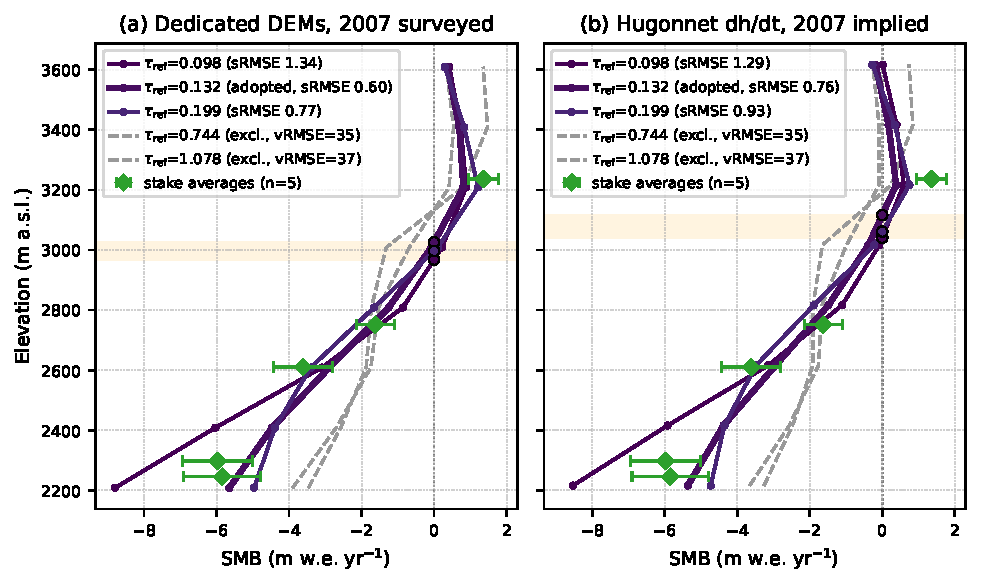
\includegraphics[width=\linewidth]{figs/fig_rhone_sens_2panel.pdf}
  \caption{Sliding-coefficient sensitivity of the Rhône inversion for two
    2007--2016 experiments sharing an identical DA state (Sect.~\ref{sec:da},
    anchored on the real 2016 DEM): (a)~the surveyed swisstopo 2007 DEM used in the
    main text and (b)~a 2007 surface implied by applying the \citet{hugonnet2021}
    $\mathrm{d}h/\mathrm{d}t$ product backward from the same 2016 DEM. Each panel
    shows the inferred SMB profile across a range of $\tau_{\mathrm{ref}}$ (colour;
    the profile at the main text's adopted $\tau_{\mathrm{ref}}=0.132$ bold with its
    stake RMSE, and runs with velsurf misfit $>1.5\times$ the panel's best rejected,
    dashed), the equilibrium-line-altitude band shaded over the retained runs, all
    validated against the \emph{same} $n=5$ 2007--2016 stake averages (green
    diamonds). Both experiments recover the elevation structure, but the
    Hugonnet-based fan sits higher and fits the stakes less well in the accumulation
    area, giving a larger stake RMSE at the adopted $\tau_{\mathrm{ref}}$ ($0.77$ vs
    $0.60\,\mathrm{m\,w.e.\,yr^{-1}}$).}
  \label{fig:hugonnet}
\end{figure*}

\subsection{Mechanical equilibrium of the calibrated dynamical state}\label{app:equilibrium}

Sect.~\ref{sec:overview} treats the DA-calibrated bedrock, sliding field and
ice-flow emulator as a fixed dynamical substrate and attributes all subsequent
thickness change over the inversion window to the free $smb(z)$ profile
(Sect.~\ref{sec:inference}). That attribution requires the substrate itself to be
close to mechanical equilibrium: if it were not, integrating it forward would
drift even under zero mass-balance forcing, and that drift would alias into the
inferred $smb$ as an initialisation shock \citep{seroussi2011}. We test this
directly on Argentière by integrating each of the two candidate starting states
for one year under $smb\equiv 0$ and measuring the resulting on-ice thickness
change: the DA-calibrated state $H_{t_2}$ itself (fit directly to the velocity
observations, Sect.~\ref{sec:da}), and the derived start-epoch state $H_{t_1}$
(Eq.~\ref{eq:hinit}) that the production run actually starts from.

Both states show a near-zero mean drift over the year ($-0.10\,\mathrm{m}$ for
$H_{t_2}$, $-0.33\,\mathrm{m}$ for $H_{t_1}$; Fig.~\ref{fig:shock}c)---an order of
magnitude below the metre-scale annual $smb$ the inversion subsequently
recovers---so neither state is spontaneously gaining or losing mass under the
calibrated dynamics: there is no systematic bias left for the $smb$ inversion to
compensate for. The drift distribution is close to symmetric about zero
(Fig.~\ref{fig:shock}c) and concentrated at a handful of margin and
tributary-confluence cells (Fig.~\ref{fig:shock}a,b) rather than spread evenly
over the glacier, consistent with local relaxation of the discretised stress
balance rather than a large-scale imbalance. In absolute terms this local
redistribution is not negligible---on-ice $\mathrm{RMS}=7.2\,\mathrm{m}$ for
$H_{t_2}$ and $9.7\,\mathrm{m}$ for $H_{t_1}$ (35\,\% larger), against the
$15.8\,\mathrm{m}$ RMS thickness change the $smb$ inversion itself fits over the
full nine-year window (Sect.~\ref{sec:results})---so we report it rather than
discount it; but its near-zero mean and localised footprint show it behaves as
noise the free $smb(z)$ parameters absorb, not as a coherent drift that would bias
the inferred mass balance. 

\begin{figure*}
  \centering
  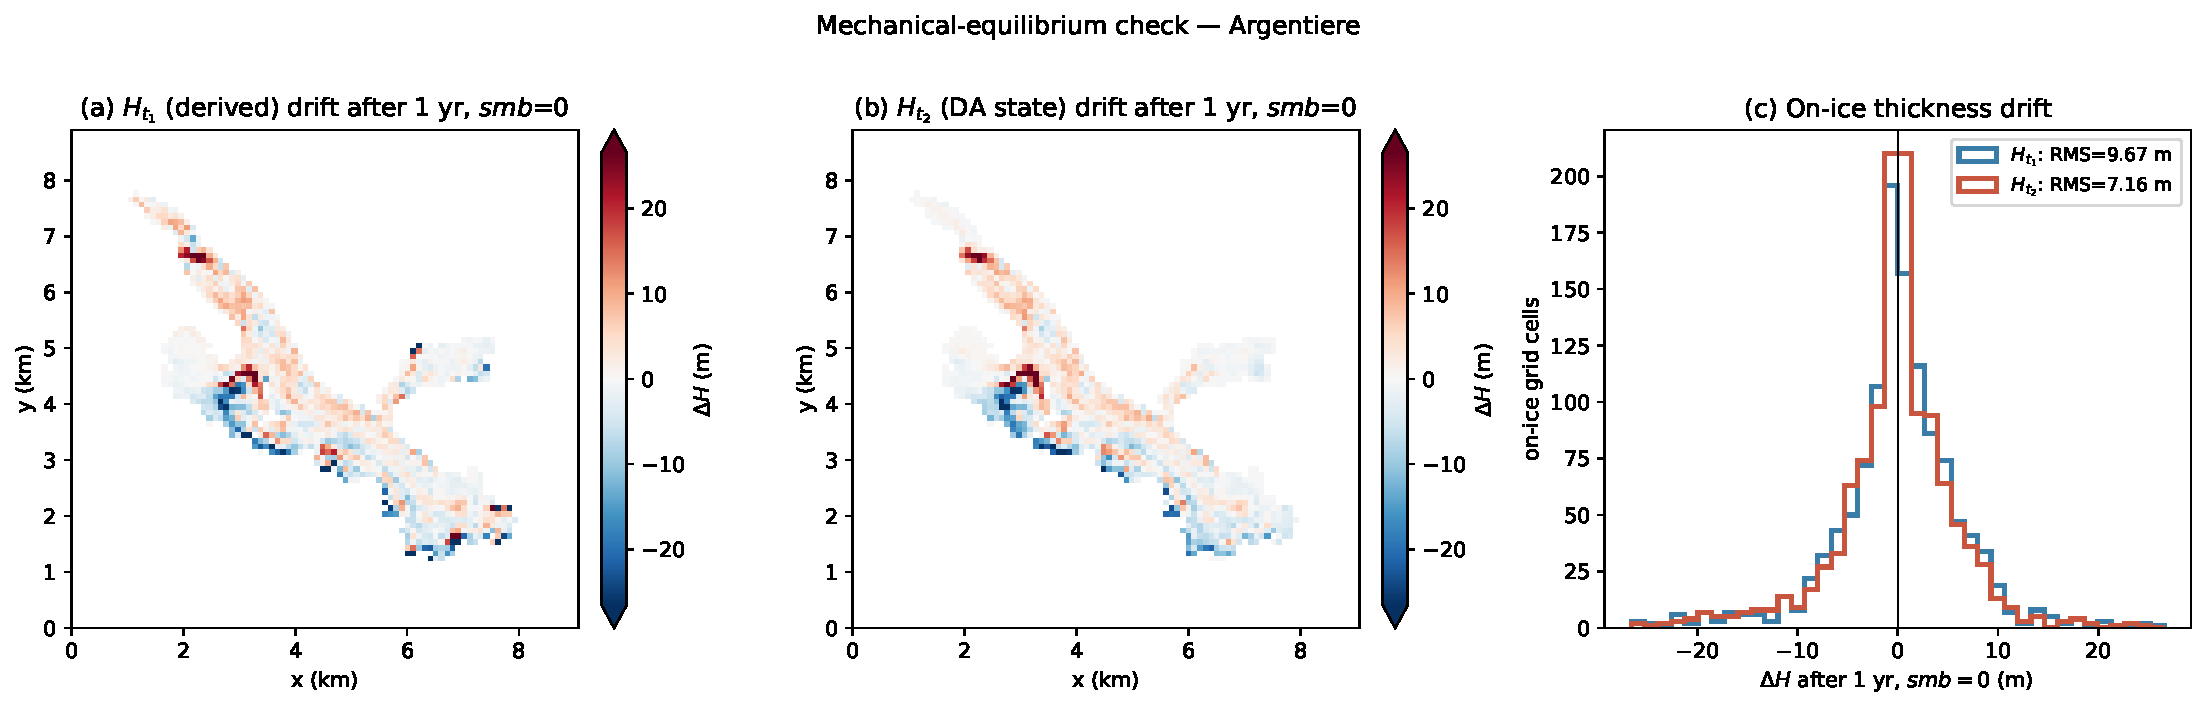
\includegraphics[width=\linewidth]{figs/fig_shock_check.pdf}
  \caption{Mechanical-equilibrium check on Argentière: on-ice thickness drift
    after integrating one year forward under $smb\equiv 0$, starting from (a) the
    derived start-epoch state $H_{t_1}$ and (b) the DA-calibrated state $H_{t_2}$;
    (c) the two drift distributions overlaid, with their on-ice RMS.}
  \label{fig:shock}
\end{figure*}
